\documentclass[11pt]{article}
\usepackage[utf8]{inputenc}

\title{The Geopolitics of Repression \\
  \large The Case of German Minority in the Soviet Union}
\author{Martin Kosík}
\date{December 2018}


\usepackage[round]{natbib}
\usepackage{graphicx}
\usepackage{amsmath}
\usepackage{enumitem}
\usepackage{booktabs}
\usepackage{breqn}

\usepackage[colorlinks=true, allcolors=blue]{hyperref}


\begin{document}

\maketitle

\begin{abstract}
    We use difference-in-differences strategy on data on political arrests by Soviet secret police to test how rise of Hitler affected the repressions of the Germans within the USSR. This is motivated by larger question of understanding how geopolitical considerations influence the attitude of a state towards minorities within its borders. The results show very weak evidence for the 
\end{abstract}

\section{Introduction}
What determines the attitude of a state toward ethnic minorities within its borders? Why are some minorities accommodated or assimilated and others are politically excluded and repressed? Futhermore,  Why the position of a state toward its minorities changes in time? For example Soviet Union largely accomodated its monorities by  for national minorities and promoting their language and culture establishing the autonomus republics. In 1930s however this radically changed when the soviet secret police started to target members

%Some studies emphasize that certain domestic institution such as democracy can decrease the likelihood of persecutions. However this does not explain why the same states often treat its ethnic minorities so differently.  For example (give example, man)...\\
%\citet{mylonas_politics_2013} argues that geopolitical concerns play inportant role. Specifically, the state is likely to choose repression and exclusion against a minority group if a external power with ethnic ties to the group is a geopolitical enemy.  
\citet{mylonas_politics_2013} argues that geopolitical concerns play important role. Specifically, state is likely to choose repression and exclusion if the ethnic minority's country of origin is seen as geopolitical enemy. The minority is then seen by the state as unreliable and  as potential fifth column in a case of conflict.  

We test this hypothesis on the case of German minority in Soviet union.
In 1933, Hitlers rise to power changed Germany from a neutral actor to ideological and geopolitical enemy in the perspective of the Soviet Union. We can then see how the repression changed before and after 1933 and compare it with other minorities. In particular, we use the individual arrests by soviet secret police (NKVD) as a dependent variable from the recently declassified archival materials and employ the difference in difference strategy. 

%First, the Soviet Union was large multiethnic state whose attitude to its minorities drastically changed throughout the year with   

%We use the case of German minority in the Soviet Union to test this hypothesis for several reason.  

%We test hypothesis put forward by Mylonas (2012) according to which the host state is likely to choose repression and exclusion if the ethnic minority's country of origin is seen as geopolitical enemy. 


%We test this hypothesis on the case of German minority in Soviet using the rise of Hitler as a change of geopolitical relations. 



\section{Literature review}
The existing literature on the use of repression by a state have mostly focused on the impact of  of domestic factors such as institutions and economic growth \citep{davenport_state_2007-1}.

As was mentioned, \citet{mylonas_politics_2013} proposes a theory how of geopolitical relations influence the attitude of a state towards its minorities. He also tests his theory with data on nation-building policies (categorized into 3 groups: accommodation, assimilation and exclusion)  toward  90 ethnic groups with information on their support by external powers in the post-World War I Balkans . However, the results of the cross-sectional regression, used in the study, might easily be biased due to omitted variables or reverse causality and we believe that our approach offers cleaner identification.

According to \citet{blaydes_state_2018}, a state will resort to collective punishment (based on ethnicity, religion or community membership) if it faces environment with highly asymmetric information in which it cannot identify the likely transgressors. The logic behind this is that the members of the community will police its members to avoid collective punishment. 

\citet{mcnamee_demographic_nodate} is methodologically and thematically closet study to ours. They analyze how the 1958 split in Soviet-China relations affected the demographic composition of the population in the Soviet-Chinese border regions.
Using difference-indifference strategy, they find that, after the split,  both states supported expulsions  of the minority group and sponsored immigration of the majority group but only in border regions without significant natural boundary (e.g. mountains). They conclude that the states use demographic engineering as a way to protect their vulnerable border against a hostile power. 

\section{Historical background}
\subsection{German–Soviet relations in the interwar period}
The relations between Weimar Germany and Soviet Union can be characterized as neutral or even cooperative. Both countries were somewhat isolated in the international system dominated by western powers (Great Britain, France, USA) and sought to find allies. The good relations were first established by the Treaty of Rappalo in 1922 in which both countries renounced the territorial and financial claims against the other and agreed to secret military cooperation and then reaffirmed by the Treaty of Berlin in 1926. Furthermore, a trade treaty was signed between the two countries in 1925 \citep{morgan_political_1963}.

Hitler was named chancellor on 30 January 1933 and effectively become a dictator on 24 March 1933 by the passing of the Enabling Act. The German Communist Party was first abolished and many of its member were send to concentratoin camps lm
The relations with Soviet Union quickly turned hostile. Hitler 

\subsection{Ethnic repressions in the Soviet Union}
In the 1920s, the Soviet policy towards its ethnic minorities was largely accommodating \citep{martin_affirmative_2001}. In some cases Autonomous Soviet Socialist Republics (ASSR) were established (including Volga German ASSR) which had given the regional minorities certain degree of independence. The languages and culture of minorities were even often promoted and minorities were encouraged to enter local goverments and party structures (so-called \emph{korenizatsiya} policy). 

This attitude changed drastically in the 1930s. First, the  \emph{korenizatsiya} policy started to be reversed. The Soviet state then gradually  began to target ethnic minorities for repressions  which culminated in the mass national operations of the NKVD of 1937-1938. The largest \citep{snyder_bloodlands:_2011}. Furthermore 

The persecutions  further escalated with the World War II. Following the German invasion into the Soviet Union in 1941, Stalin ordered deportation of about 400 000 Volga Germans into Kazakhstan and Siberia. 
\section{Data}
Our data on soviet repressions come from  \citet{zhukov_stalins_2018}\footnote{In particular, we downloaded the data from the replications file archive of the journal available  at \url{https://www.prio.org/JPR/Datasets/}} who use  the Victims of Political Terror archive  collected by a Russian NGO Memorial.The main sources of the Memorial lists are declassified Russian Interior Ministry documents, prosecutor’s offices and the Commission for the Rehabilitation of Victims of Political Repression.
 The Memorial archives include 2.6 individual arrest by the Soviet secret police (NKVD) between  the years 1921 and 1959 with names of each person, date of arrest, the place of birth for all observations and some in many cases additional information such as ethnicity, occupation and party membership. 
 However the data are not complete and include about 70\% of 3.8 million convicted under Article 58

We created our main dataset by counting number of arrest for each ethnicity by year.  A few people who were categorized as having multiple ethnicities were dropped from the dataset and not counted. 
With 17  minorities (Armenian, Belarussian, Estonian, German, Greek, Chechen, Chinese, Jewish, Kabardin, Kalmyk, Korean, Latvian, Lithuanian, Ossetian, Polish, Tatar and Ukrainian) and 37 time periods (from 1921 to 1958) this gives us 663 observations in total. The 

\section{Methodology}
We follow the standard difference-in-differences strategy
\begin{multline}
 \log\left(1 + y_{it}\right) = \lambda_t + a_i  + \delta german_{it} \cdot post_{it} + E_i \cdot t \: + \\ \sum_{k= 1}^3 \gamma_k \, german_{it} \cdot post_{it+ k} + \sum_{j= 1}^5 \omega_j \, german_{it} \cdot post_{it - k}  + u_{it}   
\end{multline}

where $y_{it}$ is number of arrests of people with ethnicity $i$ in year $t$, $\lambda$ is year fixed effect, $a$ is ethnicity fixed effect (both captured by respective dummy variables) and $post$ is a dummy that equals 0 before the year 1933 (exclusive) and 1 after it. The coefficient of interest here is $\delta$. The 5 coefficients $\omega_j$ capture the potential lagged effects (extending from 1934 to 1938), whereas the 3 coefficients capture the lead (anticipatory) effects (from 1930 to 1932) used to test pre-treatment parallel trends.  The $ E_i \cdot t$ term capture the ethnicity specific linear time trends. The inclusion of this term should not significantly  change the coefficients, unless the results are driven by spurious correlation (see Angrist. 

 We apply logarithmic transformation on $y_{it}$ since it better fits the data (more in the results below).  We use $\log\left(1 + y_{it}\right)$ because some observations (although not many) have $y = 0$. As discussed in \citet[p. 193]{wooldridge_introductory_2015},  the percentage change interpretation is usually  closely preserved (except for changes beginning at 0 which are not of interest to us).   

Our identifying assumption is that the number of arrest of Germans after 1933 would go in parallel to arrests of other minorities in the absence shock to German-Soviet relations conditional on our control variables (mainly the ethnicity specific time trends). Although we cannot test this assumption, we can test whether the trends were parallel prior to 1933 (pre-treatment) which could increase our confidence that they were parallel after 1933 too. This can be testing if the coefficients on lead effects ($\gamma_k$) are significantly different from zero.  
\section{Results}
The results of our main specification are presented in the table \ref{dif_table}, in column (1). The estimated coefficients together with their 95\% confidence  from this model are plotted in the figure \ref{fig_did_effets}. We can see that all coefficients for years 1930 to 1932 are statistically insignificant which means that the pre-treatment trends in arrests of German minority were likely parallel to the pre-treatment trends of other minorities which gives us greater  confidence in the validity of our identification strategy. 

The coefficients on all other years are insignificant as well. Only for 1934 (one year lag) is the estimate  significant at 10\% level ($p$-value of 0.13). This seems to suggest that in 1934 NKVD targeted Germans  relatively more that other minorities, the 
\begin{figure}[h]
\centering
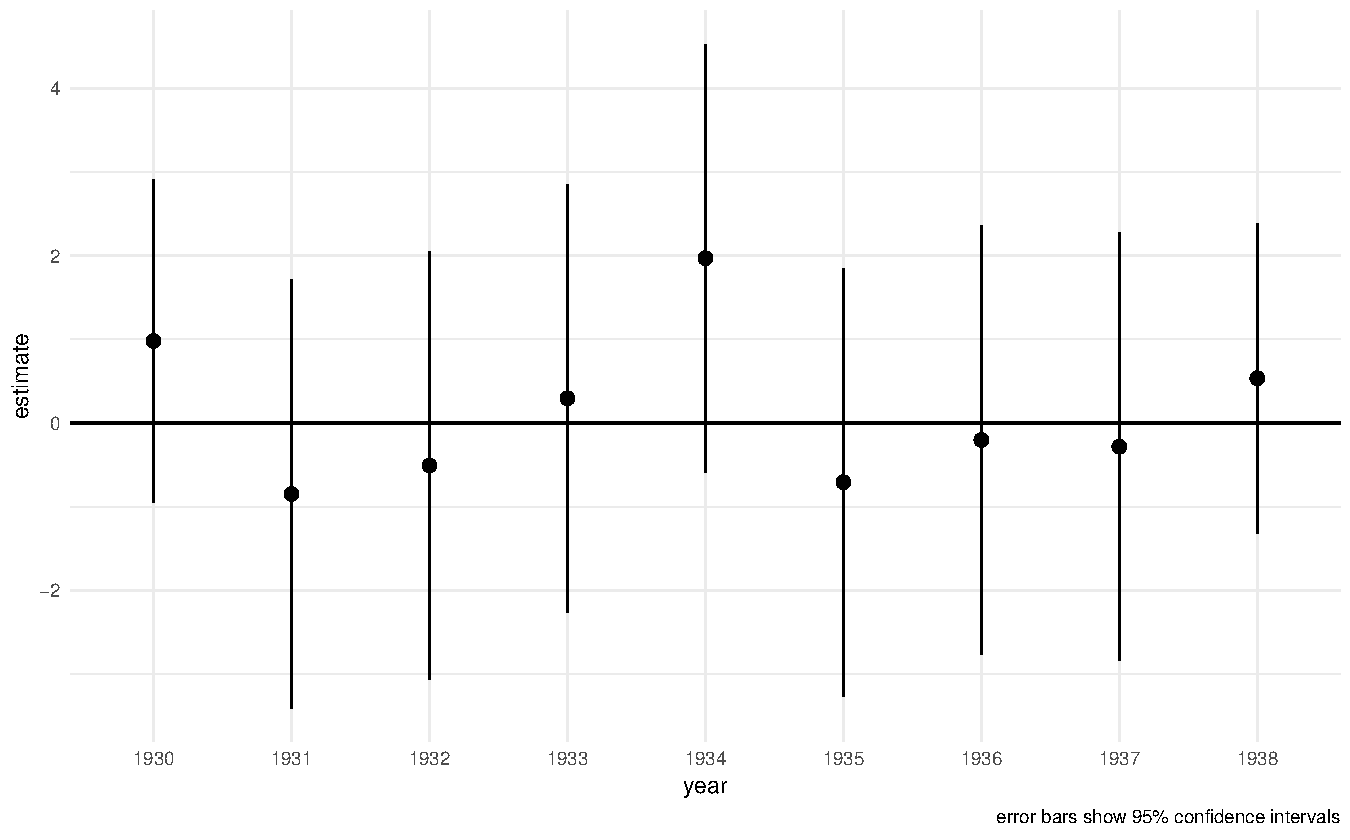
\includegraphics[width=\textwidth]{plots/did_effects.pdf}
\caption{Estimates of coefficients on $german \cdot post\_year$}
\label{fig_did_effets}
\end{figure}

We perform several robustness checks to asses sensitivity of the results to different specifications. First, in our main model, we include all observations in years 1923 to 1958. The relationship between Germany and Soviet Union were somewhat more complicated after the World War II. We thus re-estimate the model with only the data from 1923 to 1945. The results (in column (2) of table \ref{dif_table}) change only little and does not alter our previous conclusions. Second, when we omit the ethnicity specific linear time trends in column (3) we see again that the coefficients are very similar to the original model. 
Finally, we estimate a specification with number of arrests as a dependent variable (without logarithmic transformation). We can see that this model (shown in column (4)) fits the data rather poorly with  $R^2$ only of 0.411 (compared to 0.863 in the logarithmic specification).
\section{Conclusion}
We used difference-in-differences to test whether the change in geopolitical relations between Soviet Union and Germany in 1933 caused the NKVD to target Soviet Germans more relative to other minority group. One possible explanation might be that the Germans were well represented in state institutions (including the NKVD) in regions of their heavy settlements (especially in Volga German ASSR) thus would not be prone to target their co-ethnics. \citet[p. 126]{polian_against_2003} for example mentions that even on 31 June 1941, the Supreme Court of the Volga German ASSR sentenced a Russian $kolchoz$ chief for "delivering chauvinistic abuses against Germans residing in the USSR". The fruitful area for further research might be to compare how the rise in repressions differed for Germans living in areas with local autonomy (e.g. Volga German ASSR) and those living outside to see to what extent autonomy offered protection. 

We have seen that even though there was a rise in arrests in 1934 it was not statistically significant. One explanations might be that many NKVD officers were members of ethnic minorities who understood that their co-ethnics do not pose any real threat.  Polian 126


\bibliographystyle{agsm}
\bibliography{bibliography.bib}
\newpage
\section*{Appendix}
\begin{table}[!h]

\caption{\label{tab:total_arrests_by_ethnicity}Total arrest by ethnicity, 1921-1960}
\centering
\fontsize{8}{10}\selectfont
\begin{tabular}{lrrr}
\toprule
\multicolumn{1}{c}{ } & \multicolumn{3}{c}{Reference} \\
\cmidrule(l{2pt}r{2pt}){2-4}
Ethnicity & Only Labeled & Labeled + Unadj. Imputation & Labeled + Adj. Imputation\\
\midrule
Russian & 550 280 & 1 064 596 & 1 069 379\\
Belorussian & 67 613 & 85 517 & 72 979\\
Polish & 61 221 & 85 258 & 79 742\\
German & 60 798 & 168 419 & 169 955\\
Ukrainian & 54 403 & 91 814 & 97 042\\
Kazakh & 37 125 & 46 540 & 43 541\\
Tatar & 32 095 & 72 417 & 71 351\\
Jewish & 31 050 & 43 710 & 42 613\\
Latvian & 15 444 & 21 628 & 18 796\\
Chinese & 9 693 & 11 506 & 10 466\\
Estonian & 9 402 & 15 561 & 13 380\\
Chuvash & 8 910 & 14 930 & 26 520\\
Bashkir & 8 428 & 17 876 & 18 615\\
Finnish & 8 337 & 14 594 & 13 550\\
Mordvin & 6 011 & 12 682 & 20 642\\
Buryat & 5 679 & 6 735 & 6 715\\
Mari & 5 383 & 7 482 & 12 288\\
Lithuanian & 4 651 & 5 474 & 5 522\\
Karelian & 4 174 & 9 941 & 5 379\\
Korean & 4 060 & 8 821 & 11 560\\
Komi & 3 613 & 5 834 & 4 281\\
Ossetian & 3 237 & 3 724 & 3 419\\
Udmurt & 3 082 & 4 454 & 5 566\\
Armenian & 2 937 & 4 850 & 4 674\\
Kabardian & 2 733 & 4 438 & 4 021\\
Greek & 2 246 & 24 500 & 25 514\\
Khakas & 2 221 & 8 137 & 6 136\\
Altai & 1 894 & 2 477 & 2 471\\
Georgian & 1 621 & 3 049 & 1 993\\
Yakut & 1 544 & 2 909 & 1 572\\
Moldovan & 1 392 & 2 765 & 2 719\\
Kalmyk & 1 293 & 2 168 & 2 059\\
Japanese & 1 231 & 14 571 & 10 821\\
Uzbek & 1 061 & 4 044 & 7 470\\
Hungarian & 1 018 & 1 611 & 1 119\\
Bulgarian & 1 015 & 2 479 & 1 904\\
Balkar & 861 & 4 740 & 3 423\\
Chechen & 696 & 8 508 & 11 548\\
\bottomrule
\end{tabular}
\end{table}

\begin{figure}[h]
\centering
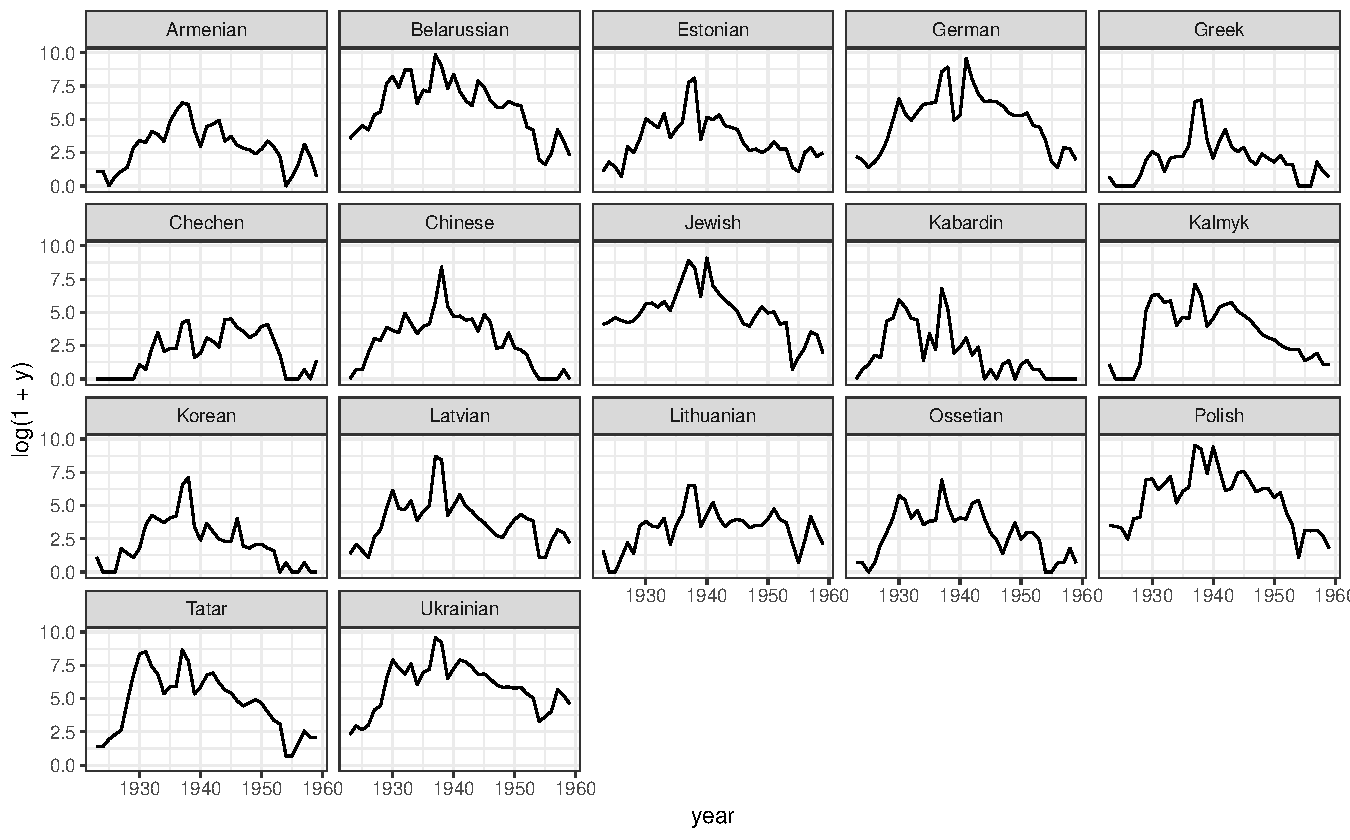
\includegraphics[width=1.2\textwidth]{plots/arrests_by_ethnicity.pdf}
\caption{Arrests by ethnicity and year (in $log(1 + y_{it})$)}
\label{fig:universe}
\end{figure}
\newpage

% Table created by stargazer v.5.2.2 by Marek Hlavac, Harvard University. E-mail: hlavac at fas.harvard.edu
% Date and time: p�, led 11, 2019 - 10:10:43
\begin{table}[!htbp] \centering 
  \caption{Difference-in-differences results} 
  \label{dif_table} 
\begin{tabular}{@{\extracolsep{5pt}}lcccc} 
\\[-1.8ex]\hline 
\hline \\[-1.8ex] 
 & \multicolumn{4}{c}{\textit{Dependent variable:}} \\ 
\cline{2-5} 
\\[-1.8ex] & \multicolumn{3}{c}{$\log(1 + y_{it})$} & $y_{it}$ \\ 
 & 1921-1958 & 1921-1945 & 1921-1945 & 1921-1958 \\ 
\\[-1.8ex] & (1) & (2) & (3) & (4)\\ 
\hline \\[-1.8ex] 
 $german*post\_1930$ & 1.196 & 0.731 & 0.855 & 683.539 \\ 
  & (0.887) & (0.984) & (0.963) & (1,495.164) \\ 
  & & & & \\ 
 $german*post\_1931$ & $-$0.779 & $-$0.872 & $-$0.847 & $-$61.209 \\ 
  & (1.177) & (1.198) & (1.292) & (1,983.046) \\ 
  & & & & \\ 
 $german*post\_1932$ & $-$0.439 & $-$0.532 & $-$0.507 & 63.854 \\ 
  & (1.177) & (1.198) & (1.292) & (1,983.046) \\ 
  & & & & \\ 
 $german*post\_1933$ & 0.365 & 0.272 & 0.297 & 199.791 \\ 
  & (1.177) & (1.198) & (1.292) & (1,983.046) \\ 
  & & & & \\ 
 $german*post\_1934$ & 2.040$^{*}$ & 1.947 & 1.971 & 996.604 \\ 
  & (1.177) & (1.198) & (1.292) & (1,983.046) \\ 
  & & & & \\ 
 $german*post\_1935$ & $-$0.638 & $-$0.731 & $-$0.706 & 49.979 \\ 
  & (1.177) & (1.198) & (1.292) & (1,983.046) \\ 
  & & & & \\ 
 $german*post\_1936$ & $-$0.134 & $-$0.227 & $-$0.202 & 71.041 \\ 
  & (1.177) & (1.198) & (1.292) & (1,983.046) \\ 
  & & & & \\ 
 $german*post\_1937$ & $-$0.214 & $-$0.307 & $-$0.282 & 637.291 \\ 
  & (1.177) & (1.198) & (1.292) & (1,983.046) \\ 
  & & & & \\ 
 $german*post\_1938$ & 1.322 & 0.772 & 0.537 & 2,304.034 \\ 
  & (0.906) & (0.972) & (0.934) & (1,526.238) \\ 
  & & & & \\ 
\hline \\[-1.8ex] 
Year dummies & Yes & Yes & Yes & Yes \\ 
Ethnicity dummies & Yes & Yes & Yes & Yes \\ 
Ethnicity time trends & Yes & Yes & No & Yes \\ 
Observations & 663 & 425 & 663 & 663 \\ 
R$^{2}$ & 0.890 & 0.900 & 0.864 & 0.428 \\ 
Adjusted R$^{2}$ & 0.875 & 0.882 & 0.850 & 0.350 \\ 
\hline 
\hline \\[-1.8ex] 
\textit{Note:}  & \multicolumn{4}{r}{$^{*}$p$<$0.1; $^{**}$p$<$0.05; $^{***}$p$<$0.01} \\ 
\end{tabular} 
\end{table} 

\thispagestyle{empty}

\end{document}
